%%
%% Capítulo 2: Regras gerais de estilo
%%

\mychapter{Fundamentação Teórica}
\label{Cap:Teoria}

\section{O problema da cinemática de um robô móvel}
Dado um robô de acionamento diferencial, onde a velocidade
angular das $n$ rodas são: $\phi_0,\phi_1,\phi_2,...,\phi_n$.
Uma cinemática direta $f$ de um robô móvel é a uma função que mapeia as velocidades
angulares das rodas para a velocidade linear $v$ e velocidade angular $\omega$
do robô, $f(\phi_0,\phi_1,\phi_2,...,\phi_n) \rightarrow v,\omega$. Já
a cinemática inversa $g$, mapeia a velocidade angular e linear do robô para, um
conjunto de velocidades angulares das rodas, $g(v,\omega) \rightarrow  \phi_0,\phi_1,\phi_2,...,\phi_n$.
cinemática é portanto um conjunto de regras que relaciona a velocidade linear e angular
com as velocidades das rodas.

\begin{figure}[H]
    \centering
    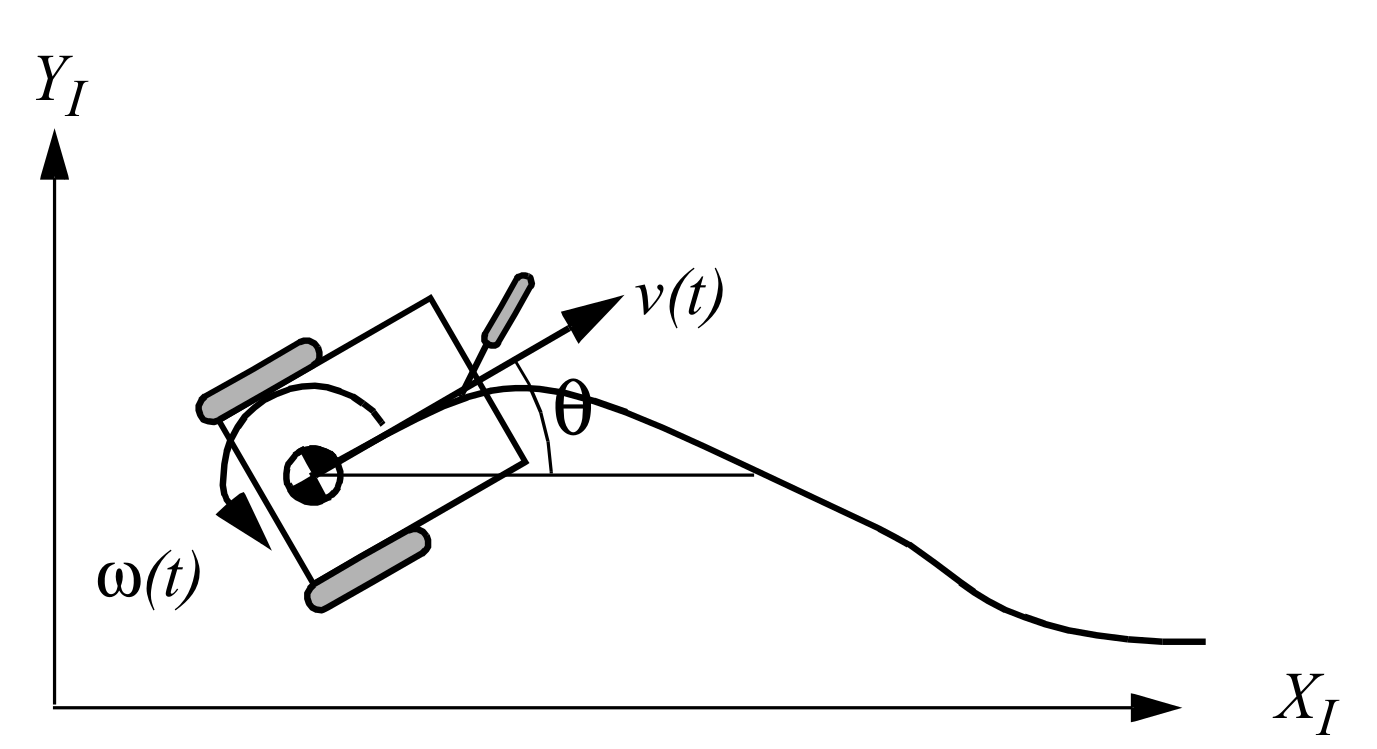
\includegraphics[scale=0.9]{figuras/robo.png}
    \caption[]{Robô móvel com acionamento diferencial}
\end{figure}

A cinemática de um robô móvel está fortemente relaciona a modelagem
das rodas do robô, de forma geral chega-se os seguintes sistemas
afim: $L_r\times v_r +B_r = \phi_r$ e $K_r \times v_r + C_r = 0$

\[
\begin{bmatrix}
    A_{11}sen(W_{11}\alpha_{11} + \beta_{11}) &  A_{12}sen(W_{12}\alpha_{12} + \beta_{12}) &  A_{13}sen(W_{13}\alpha_{13} + \beta_{13})\\
    A_{21}sen(W_{21}\alpha_{21} + \beta_{21}) &  A_{22}sen(W_{22}\alpha_{22} + \beta_{22}) &  A_{23}sen(W_{23}\alpha_{23} + \beta_{23})\\
    \vdots & \vdots & \vdots \\
    A_{n1}sen(W_{n1}\alpha_{n1} + \beta_{n1}) &  A_{n2}sen(W_{n2}\alpha_{n2} + \beta_{n2}) &  A_{n3}sen(W_{n3}\alpha_{n3} + \beta_{n3})\\
\end{bmatrix}
\begin{bmatrix}
    v_x \\
    v_y \\
    \omega\\
\end{bmatrix}
+
\begin{bmatrix}
    B_0 \\
    B_1 \\
    \vdots \\
    B_n \\
\end{bmatrix}
=
\begin{bmatrix}
    \phi_0 \\
    \phi_1 \\
    \vdots \\
    \phi_n \\
\end{bmatrix}
\]
\newpage

\[
\begin{bmatrix}
    D_{11}sen(Q_{11}\gamma_{11} + \mu_{11}) &  D_{12}sen(Q_{12}\gamma_{12} + \mu_{12}) &  D_{13}sen(Q_{13}\gamma_{13} + \mu_{13})\\
    D_{21}sen(Q_{21}\gamma_{21} + \mu_{21}) &  D_{22}sen(Q_{22}\gamma_{22} + \mu_{22}) &  D_{23}sen(Q_{23}\gamma_{23} + \mu_{23})\\
    \vdots & \vdots & \vdots \\
    D_{n1}sen(Q_{n1}\gamma_{n1} + \mu_{n1}) &  D_{n2}sen(Q_{n2}\gamma_{n2} + \mu_{n2}) &  D_{n3}sen(Q_{n3}\gamma_{n3} + \mu_{n3})\\
\end{bmatrix}
\begin{bmatrix}
    v_x \\
    v_y \\
    \omega\\
\end{bmatrix}
+
\begin{bmatrix}
    C_0 \\
    C_1 \\
    \vdots \\
    C_n \\
\end{bmatrix}
=
\begin{bmatrix}
    0 \\
    0 \\
    \vdots \\
    0 \\
\end{bmatrix}
\]
onde $A$, $D$, $W$, $Q$, $B$, $C$, $\alpha$, $\gamma$, $\beta$, $\mu$
são propriedades das rodas do robô. $v_x$,$v_y$ são as velocidade lineares
do robô  e $\omega$ é a velocidade angular do robô.  É importante salientar
que os parâmetros das rodas são extraídos seguindo o referencial do robô $X_r$,$Y_r$.
Caso a velocidade linear do robô for medida em outro referencial, é necessário
fazer uma rotação do referencial medido para a orientação do robô
\begin{figure}[H]
    \centering
    % 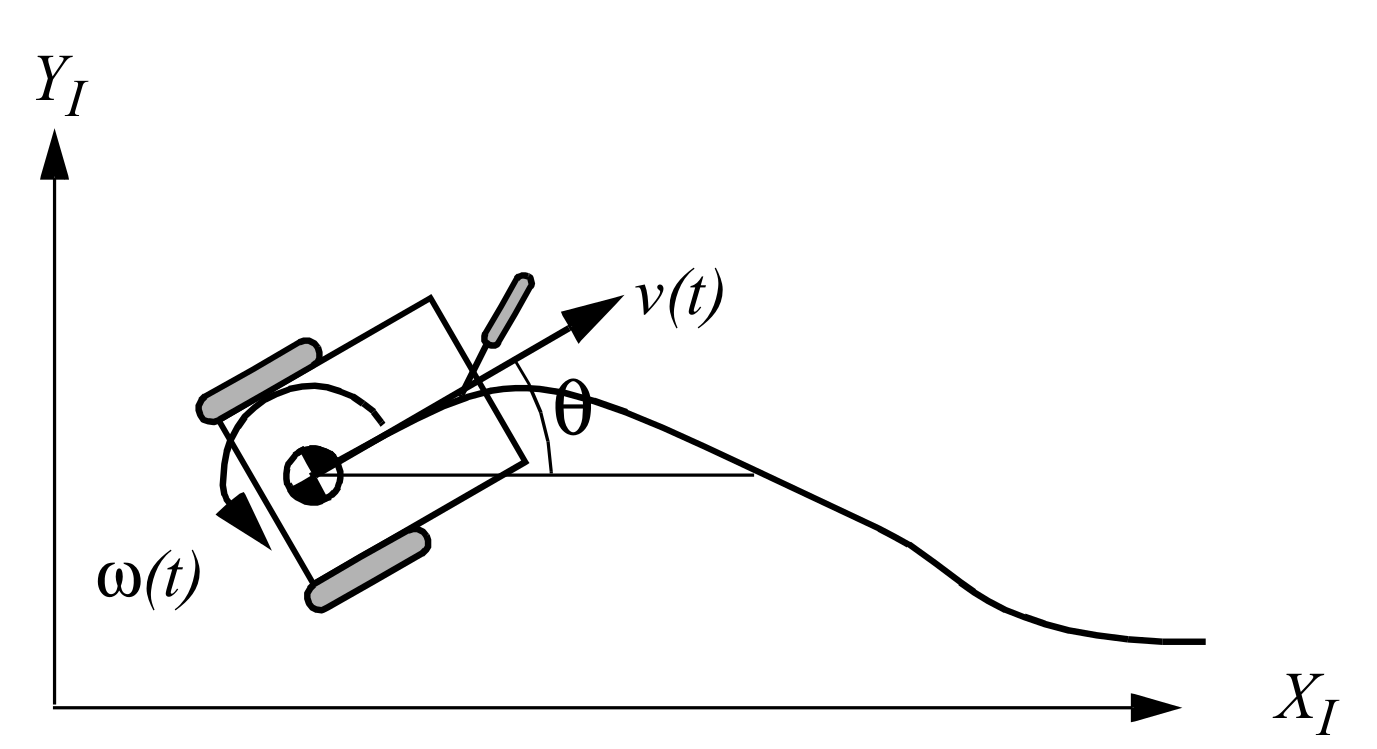
\includegraphics[scale=0.9]{figuras/robo.png}
    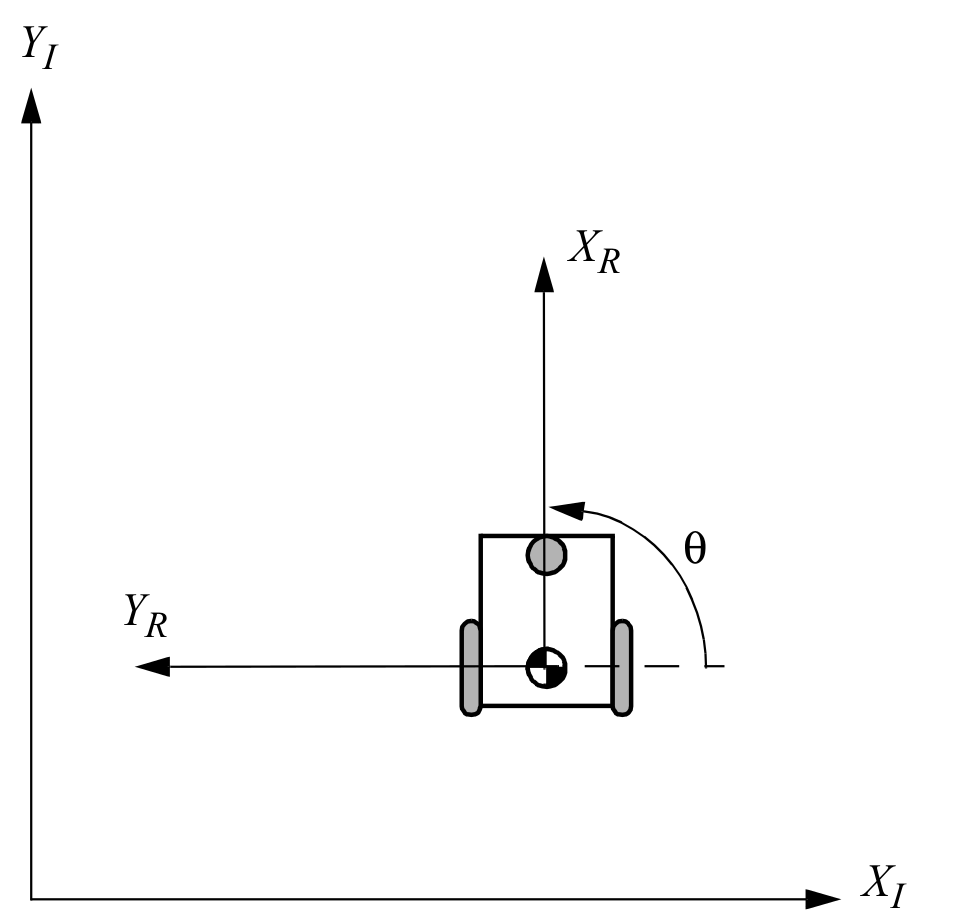
\includegraphics[scale=0.3]{figuras/robo_coordenadas.png}
    \caption[]{Mudança de referencial}
\end{figure}

\[
    \begin{bmatrix}
        v_x \\
        v_y \\
        \omega
    \end{bmatrix}
    =
    \begin{bmatrix}
        cos(\theta)  & sin(\theta) & 0 \\
        -sin(\theta) & cos(\theta) & 0 \\
        0 & 0 & 1 \\
    \end{bmatrix}
    \begin{bmatrix}
        v_{x_I} \\
        v_{y_I} \\
        \omega
    \end{bmatrix}
\]

onde $v_{x_I}, v_{y_I}$, são as velocidades no referencial $X_I,Y_I$.
\newpage

No nosso caso, o robô a ser modelado possui quatro rodas, duas delas são
rodas tratore e as outras duas rodas, são rodas castores. Apesar das rodas
castores, contribuírem para o movimento, elas não restringem o movimento,
portanto podemos entender o modelo cinemático do nosso robô como sendo
uma transformação afim $W \times X + B = Y$, onde $X$ são as entradas
do nosso modelo cinemático, $W$ e $B$ são parâmetros das
rodas que devido a modelagem e a construção do robô, são parâmetros
constantes. No nosso robô, caso queremos calcular a cinemática direta
a entrada $X$ são as velocidades das rodas do robô e $Y$ a velocidade
linear e angular do robô, caso queiramos calcular a cinemática inversa
do robô, $X$ são as velocidades lineares e a velocidade angular do robô
e $Y$ as velocidades da rodas. Neste trabalho visamos criar um controlador
para o robô e como o controlador enviará um sinal de velocidade linear
e angular para a cinemática, portanto queremos a cinemática inversa
do nosso robô.

\begin{figure}[H]
    \[
    \begin{bmatrix}
        W_{11} &  W_{12} & W_{13} \\
        W_{21} &  W_{22} & W_{23} \\
    \end{bmatrix}
    \begin{bmatrix}
        v_x \\
        v_x \\
        \omega \\
    \end{bmatrix}
    +
    \begin{bmatrix}
        B_{1} \\
        B_{2} \\
    \end{bmatrix}
    =
    \begin{bmatrix}
        \phi_{\text{left}} \\
        \phi_{\text{right}} \\
    \end{bmatrix}
\]
    \caption{Cinemática inversa}
\end{figure}


\begin{figure}[H]
    \centering
    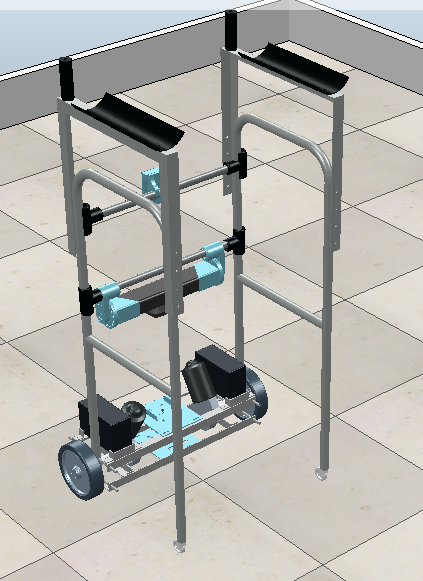
\includegraphics[scale=0.4]{figuras/smart_walker.png}
    \caption{Andador inteligente}
\end{figure}

\section{Aprendizado de máquina}
Usualmente quando programamos computadores para
resolver determinada tarefa, nos codificamos as regras e
executamos o programa com os dados de entrada, esta é a abordagem clássica
de se resolver um problema. Uma outra forma de usar computadores
é criar sistemas como aprendizado máquina, onde nós possuímos os
dados de entrada necessários, as respontas e queremos que a máquina retorne
para nós quais são as regras que transformam os dados nas respostas
desejadas \cite{chollet2021deep}.

\begin{figure}[H]
    \centering
    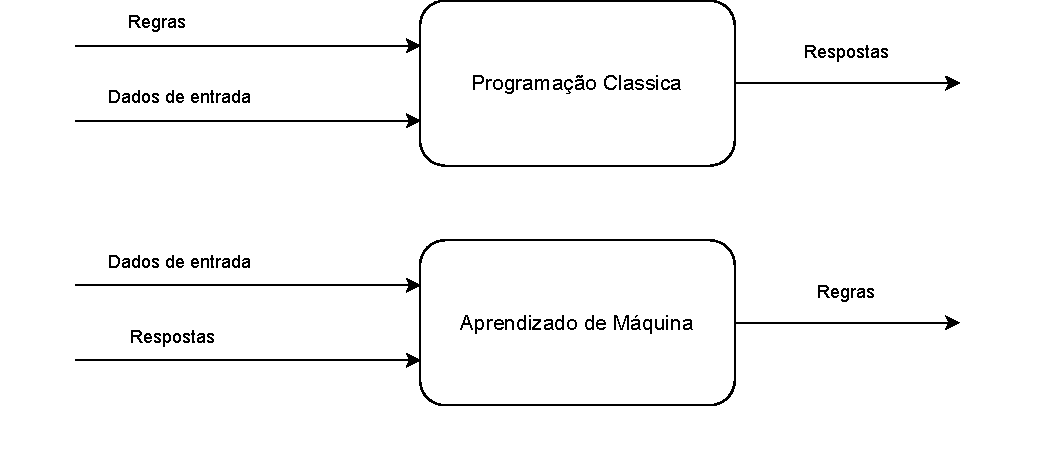
\includegraphics[scale=0.7]{figuras/machine_learning_diagram.pdf}
    \caption{Aprendizado de máquina e Programação clássica}
\end{figure}

Existem três tipos de aprendizado de máquina, aprendizado por reforço,
aprendizado supervisionado e aprendizado não supervisionado.
Aprendizado por reforço é o aprendizado de como mapear situações
para ações de modo que maximize um sinal de recompensa
\cite{sutton2018reinforcement}. Aprendizado supervisionado é o
tipo de aprendizado onde a máquina busca extrair padrões nos conjuntos
de dados de entrada  e do conjunto de dados das respontas de modo que
transforme um dado de entrada na resposta desejada, já aprendizado não
supervisionado também buscar encontrar padrões entre os conjuntos de
dados de entrada e resposta, mas sem ter uma responta correta
\cite{trask2019grokking}. Neste trabalho foi utilizado algoritmos de
aprendizado de máquina supervisionado com objetivo de extrair um modelo de
cinemática inversa do robô andador inteligente.

\begin{figure}[H]
    \centering
    \includegraphics[scale=0.7]{figuras/aprendizado_cinemática_inversa.pdf}
    \caption{Aprendizado de máquina no calculo da cinemática inversa}
\end{figure}

Os algoritmos de aprendizado supervisionado utilizado neste trabalho
foram o Backpropagation e uma variação do algoritmo decida do gradiente, chamada
RMSprop.
Dado uma função $L(M)$, onde $L$ é uma função continua e derivável,
a decida do gradiente é uma busca que visa encontrar
a melhor matriz $M$ que minimiza uma função $L(M)$, basicamente a
decida do gradiente parte do suposto que existe a sequência
$M_0$, $M_1$, $M_2$, ..., $M_i$, $M_{i+1}$ até $M_k$, onde quando
chegar até $M_k$, o erro $L(M_k)$ será um ponto de mínimo e a transição
entre o $M_{i}$ até $M_{i+1}$, segue a seguinte regra:

\begin{figure}[H]
    \[
        M_{i+1} = M_i -\alpha \nabla L(M_i)
    \]
    \caption{Equação da decida do gradiente}
\end{figure}

onde $\nabla L(W)$ é o gradiente da função erro em relação $M$ aplicado
a $M_i$ e $\alpha$ é um número que varia de 0 até 1,
também conhecido com taxa de aprendizado. Uma variação desse algoritmo
basicamente utilizado é chamado RMSprop, ele se inspira na ideia de momentum
da física  onde  é adicionado uma constante $m$ análoga a massa e uma grandeza
vetorial $v_{\text{vel}}$ análoga a velocidade, criando uma nova equação de decida:

\begin{figure}[H]
    \begin{align*}
        v_{\text{vel}_t} = \alpha v_{\text{vel}_{t-1}} + (1 - \alpha)\nabla L(M_i)^2 \\
        b_t = mb_{t-1} + \frac{\nabla L(M_i)}{\sqrt{v_{\text{vel}_t} + \epsilon}} \\
        M_{i+1} = M_i - b_t
    \end{align*}
    \caption{Equações do RMSprop}
\end{figure}

As variáveis $v_{\text{vel}_t}$ e  $b_t$, são inicializadas como zero, pode acontecer
que  $\sqrt{v_{\text{vel}_t}}$ seja zero ou bem próximo disso então para não ter uma equação
divida por zero é adicionado uma variável $\epsilon =10^{-8}$, deixando o algoritmo numericamente
mais estável. Em contexto de aprendizado supervisionado a função $L$ é uma função erro que a
partir do Backpropagation, encontra-se os gradientes dos parâmetros de um modelo a partir
de pontos $X$ e $Y$ coletados, partindo de  uma definição de um modelo como por exemplo uma
transformação geométrica $Y_{\text{pred}}= A \times X + B$, e uma definição de uma função
erro como: $L=(Y_{\text{true}}- Y_{\text{pred}})^2$ podemos utilizar o algoritmo
Backpropagation para encontrar os gradientes da função $L$ em relação a $A$
e  $B$, basicamente o Backpropagation executa automaticamente a regra da cadeia
para encontrar os gradientes e com os gradientes podemos executar o RMSprop.

\begin{figure}[H]
    \begin{align*}
        \frac{dL}{dA } = \frac{dL}{dY_{\text{pred}} } \frac{dY_{\text{pred}}}{dA}  \\
        \frac{dL}{dB } = \frac{dL}{dY_{\text{pred}} } \frac{dY_{\text{pred}}}{dB} 
    \end{align*}
    \caption{Regra da cadeia aplicada ao modelo: $Y_{\text{pred}}= A \times X + B$ }
\end{figure}



\section{Controlador estabilizante Federico}
Controladores cinemáticos ou controladores de movimento, podem ser 
divididos em dois tipos, seguidores de trajetória e retroalimentação,
controladores seguidores trajetória recebem como entrada um perfil
de caminho sobre o tempo, a qual o controlador envia sinais de
velocidade linear e angular para o robô de modo que ele siga a
trajetória idealizada, já controladores de retroalimentação
eles recebem como entrada um estado atual do robô e o estado desejado
e buscam enviar sinais de velocidade linear e angular com o objetivo
de minimizar o erro entre o estado atual e desejado. Neste trabalho
foi utilizado um controlador de retroalimentação criado por Frederico
\cite{vieira2006controle}, o controlador recebe como entrada a posição
x,y $p_c$, orientação $\theta_c$ atual do robô e uma posição desejada $p_d$
e enviar sinais de velocidade linear $v$ e angular $\omega$ com o
objetivo de estabilizar o robô no ponto desejado.

\begin{figure}[H]
    \centering
    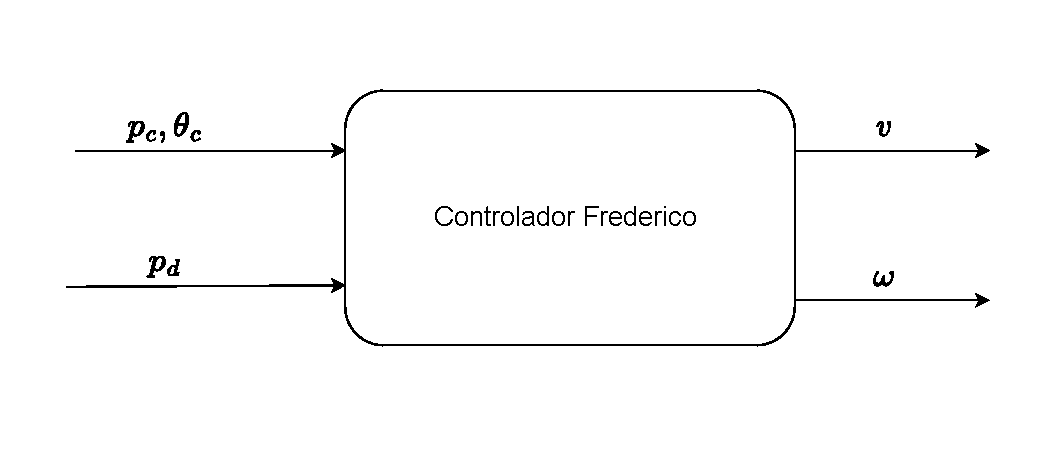
\includegraphics[scale=0.8]{figuras/controlador_frederico.pdf}
    \caption{Bloco controlador Frederico}
\end{figure}

Internamente o controlador utiliza  dois controladores proporcionais
integrais derivativos (P.I.D), um controlador é responsável pela velocidade linear $v$
e outro controlador é responsável pela velocidade angular $\omega$. 
Um controlador P.I.D é definido pela a seguinte função de
transferência $C(s)$ no domínio continuo $s$

\begin{figure}[H]
    \[
        C(s) = K_p + \frac{K_i}{s} + K_ds
    \]
    \caption{Função de transferência de um controlador P.I.D }
\end{figure}
onde $K_p$,$K_i$,$K_d$ são constantes que podem ser adquiridas ou
através da experimentação ou uma analise matemática \cite{ogataengenharia}. Para gerar sinais
velocidades $v$ e $\omega$,  o controlador Federico funciona da seguinte
maneira, primeiro é calculado o vetor posição $p_{\text{diff}}$:
\[
    p_{\text{diff}} = p_d - p_c 
\]
segundo é calculado suas coordenadas polares $l$, $\alpha$:

\[
    l = \sqrt{p_{\text{diff}_x}^2 + p_{\text{diff}_y}^2}
\]

\[
    \alpha =  \arctan(\frac{ p_{\text{diff}_y}}{p_{\text{diff}_x}}) 
\]

onde $p_{\text{diff}_x}$,$p_{\text{diff}_y}$ são as coordenadas x,y
do vetor $p_{\text{diff}}$. Terceiro é calculado o angulo $\gamma$:

\[
    \gamma =  \alpha - \theta
\]


por fim o controlador P.I.D de velocidade
linear, buscar enviar um sinal $v$ que para tender o valor $l \cos(\gamma)$
a zero e o controlador de velocidade angular busca enviar um sinal $\omega$
para  tender o valor de $\gamma$ a zero. perceba que quando o valor de $\gamma$
chega próximo a zero, da velocidade linear vai tender a reduzir a
distância $l$. Como o modelo cinemático do robô espera receber como entrada
um vetor de velocidade linear em coordenadas cartesianas então é preciso
transformar de volta a velocidade $v$ 

\[
    \begin{bmatrix}
        v_x \\
        v_y \\
    \end{bmatrix}
    =
    \begin{bmatrix}
        v\cos(\theta) \\
        v\sin(\theta) \\
    \end{bmatrix}
\]
onde, $v_x$, $v_y$ são as velocidade lineares em coordenadas cartesianas.